% \VignetteIndexEntry{R4RNA}
% \VignetteDepends{R4RNA}
% \VignetteKeywords{RNA secondary structure arc diagram visualization}
% \VignettePackage{R4RNA}

\documentclass[letterpaper]{article}
\usepackage{graphicx}
\usepackage{wrapfig}
\usepackage{fullpage}
\usepackage{hyperref}
\usepackage{caption}

\title{R4RNA: A R package for RNA visualization and analysis}
\author{Volodymyr Tsybulskyi, Mohamed Mounir, Daniel Lai,Irmtraud M.~Meyer}
\date{\today}

\usepackage{Sweave}
\begin{document}
\Sconcordance{concordance:R4RNA.tex:R4RNA.Rnw:%
1 16 1 1 0 23 1 1 2 1 0 1 2 2 1 1 2 2 1 1 2 3 1 3 0 1 2 2 1 1 3 2 0 1 1 %
1 2 1 0 3 1 1 2 5 0 2 1 1 2 5 0 1 1 6 0 1 2 7 1 1 2 1 0 1 1 4 0 1 2 4 1 %
1 2 1 0 1 1 4 0 1 2 1 1 1 2 1 0 1 1 4 0 1 2 6 1 1 2 1 0 2 1 4 0 2 2 1 0 %
2 1 4 0 1 2 1 3 2 0 2 1 4 0 1 2 6 1 1 2 1 0 1 1 3 0 1 2 3 1 1 2 1 0 1 1 %
1 2 1 1 1 3 5 0 1 2 2 1 1 2 1 0 1 1 1 2 1 1 1 3 5 0 2 2 1 0 1 1 1 2 1 1 %
1 3 5 0 1 2 10 1 1 2 5 0 1 2 2 1 1 4 3 0 2 1 4 0 1 2 1 4 3 0 2 1 4 0 1 %
2 14 1 1 2 1 0 3 1 1 2 1 1 4 0 1 2 2 1 1 2 1 0 2 1 1 2 1 3 6 0 1 2 1 1 %
1 2 1 0 2 1 1 2 1 3 6 0 1 2 10 1 1 6 10 0 1 3 2 1 1 6 9 0 1 2 3 1 1 6 9 %
0 1 2 8 1 1 2 5 0 1 2 2 1 1 2 1 0 2 1 2 2 5 0 2 2 1 0 2 1 2 2 5 0 1 2 8 %
1 1 2 1 0 1 1 1 2 5 0 1 2 1 3 1 0 2 2 5 0 1 2 3 1 1 2 1 0 1 2 1 0 1 2 5 %
0 2 2 1 0 1 5 4 0 1 2 5 0 1 2 3 1 1 2 1 0 1 1 1 2 5 0 2 2 1 0 1 1 1 2 5 %
0 1 2 3 1 1 2 1 0 1 3 6 0 2 2 1 0 1 1 4 0 1 2 4 1 1 2 1 0 1 1 3 0 1 2 3 %
1 1 2 1 0 2 1 3 0 1 2 2 1 1 2 5 0 1 2 2 1 1 2 5 0 1 2 4 1 1 2 11 0 1 3 %
1 1}


\setkeys{Gin}{width=\textwidth}

\maketitle
\tableofcontents

\section{R4RNA}

The R4RNA package aims to be a general framework for the analysis of RNA
secondary structure and comparative analysis in R, the language so chosen due
to its native support for publication-quality graphics, and portability across
all major operating systems, and interactive power with large datasets.

To demonstrate the ease of creating complex arc diagrams, a short example is
as follows.

\subsection{Reading Input}

Currently, supported input formats include dot-bracket, connect, bpseq, and a
custom ``helix'' format.  Below, we read in a structure predicted by TRANSAT,
the known structure obtained form the RFAM database.

\begin{Schunk}
\begin{Sinput}
> library(R4RNA)
> message("TRANSAT prediction in helix format")
> transat_file <- system.file("extdata", "helix.txt", package = "R4RNA")
> transat <- readHelix(transat_file)
> message("RFAM structure in dot bracket format")
> known_file <- system.file("extdata", "vienna.txt", package = "R4RNA")
> known <- readVienna(known_file)
> message("Work with basepairs instead of helices for more flexibility")
> message("Breaks all helices into helices of length 1")
> transat <- expandHelix(transat)
> known <- expandHelix(known)
\end{Sinput}
\end{Schunk}

For multiple entities you can use just updated ``helix'' format. Below, we read predicted and known structures.

\begin{Schunk}
\begin{Sinput}
> #read fasta
> fasta_file.mltp <- system.file("extdata", "fasta.mltp.txt", package = "R4RNA")
> fasta.mltp <- readBStringSet(fasta_file.mltp)
> #read helix
> transat.file.mltp <- system.file("extdata", "transat.helix.mltp.txt" ,package = "R4RNA")
> helix.transat.mltp <- readHelixMltp(transat.file.mltp)
> known.file.mltp <- system.file("extdata", "known.helix.mltp.txt", package = "R4RNA")
> helix.known.mltp <- readHelixMltp(known.file.mltp)
> is.helix.mltp(helix.transat.mltp)
\end{Sinput}
\begin{Soutput}
[1] TRUE
\end{Soutput}
\begin{Sinput}
> helix.transat.exp <- expandHelixMltp(helix.transat.mltp)
> helix.known.exp <- expandHelixMltp(helix.known.mltp)
> is.helix.mltp(helix.transat.exp)
\end{Sinput}
\begin{Soutput}
[1] TRUE
\end{Soutput}
\begin{Sinput}
> is.helix.mltp(helix.known.exp)
\end{Sinput}
\begin{Soutput}
[1] TRUE
\end{Soutput}
\end{Schunk}


\subsection{Basic Arc Diagram}

The standard arc diagram, where the nucleotide sequence is the horizontal
line running left to right from 5' to 3' at the bottom of the diagram.  Any
two bases that base-pair in a secondary structure are connect with an arc.

\begin{Schunk}
\begin{Sinput}
> plotHelix(known, line = TRUE, arrow = TRUE)
> mtext("Known Structure", side = 3, line = -2, adj = 0)
\end{Sinput}
\end{Schunk}
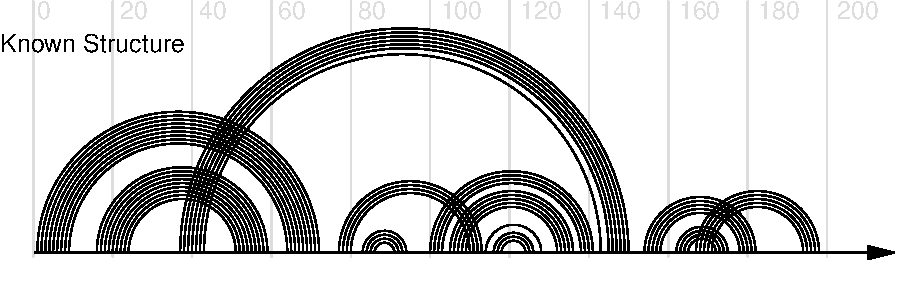
\includegraphics{R4RNA-003}

Plot for multiple entities. Trans interactions are given by length equal 1.
There is Single line and Double Line Modes.
Single line:

\begin{Schunk}
\begin{Sinput}
> plotHelixMltpSingleLine(copy(helix.known.exp),scale = FALSE)
> mtext("Known Structure", side = 3, line = -2, adj = 0)
\end{Sinput}
\end{Schunk}
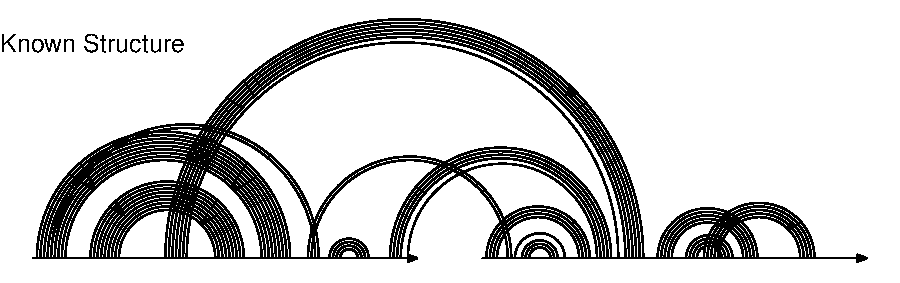
\includegraphics{R4RNA-004}

Double line:
\begin{Schunk}
\begin{Sinput}
> plotHelixMltpDoubleLine(copy(helix.known.exp),scale = FALSE)
> mtext("Known Structure", side = 3, line = -10, adj = 0)
\end{Sinput}
\end{Schunk}

\includegraphics{R4RNA-005}


\subsection{Multiple Structures}

Two structures for the same sequence can be visualized simultaneously, allowing
one to compare and contrast the two structures.

\begin{Schunk}
\begin{Sinput}
> plotDoubleHelix(transat, known, line = TRUE, arrow = TRUE)
> mtext("TRANSAT\nPredicted\nStructure", side = 3, line = -5, adj = 0)
> mtext("Known Structure", side = 1, line = -2, adj = 0)
\end{Sinput}
\end{Schunk}
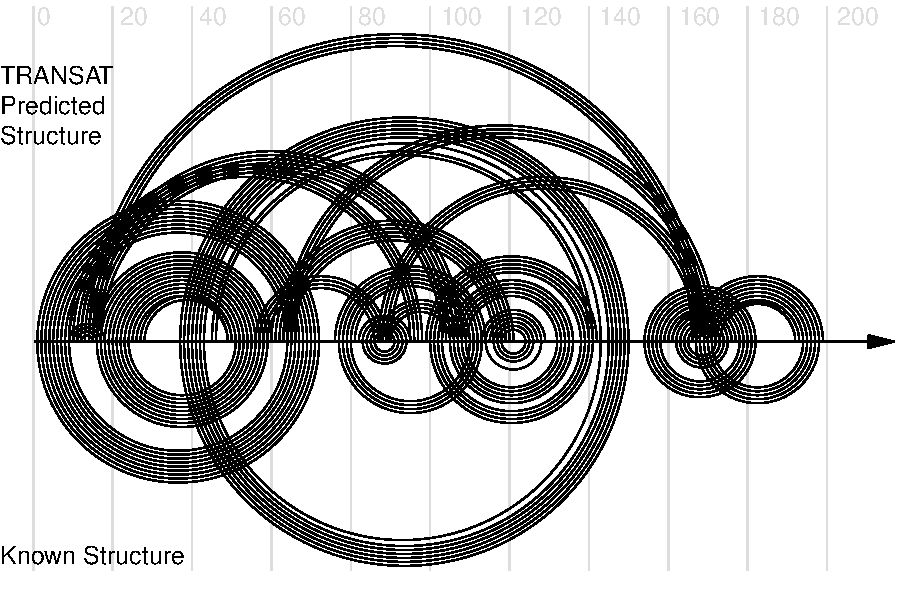
\includegraphics{R4RNA-006}

\begin{Schunk}
\begin{Sinput}
> plotDoubleHelixMltpSingleLine(helix.known.exp,helix.transat.exp,scale = FALSE)
> mtext("Predicted\nStructure", side = 1, line = -5, adj = 0)
> mtext("Known Structure", side = 3, line = -2, adj = 0)
\end{Sinput}
\end{Schunk}
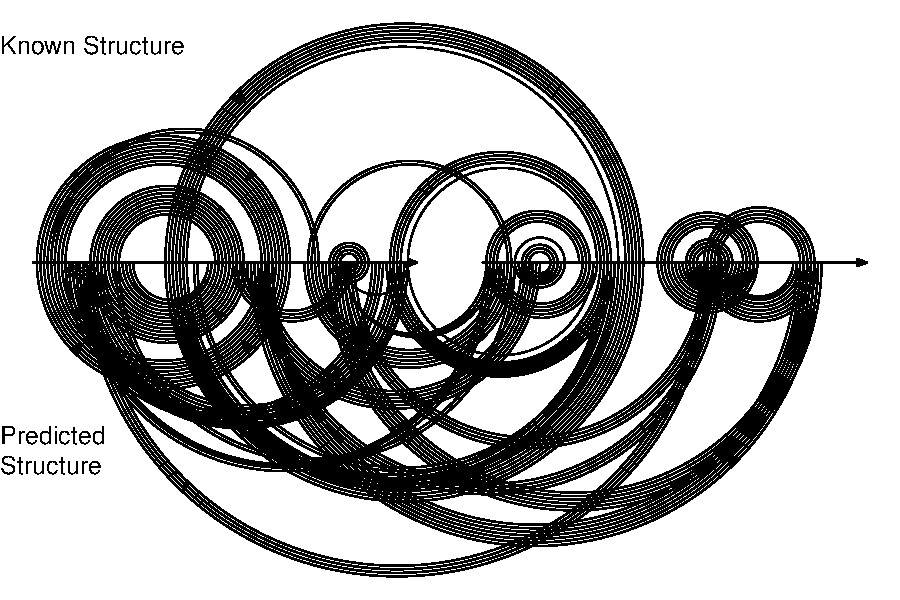
\includegraphics{R4RNA-007}

\begin{Schunk}
\begin{Sinput}
> plotDoubleHelixMltpDoubleLine(helix.known.exp,helix.transat.exp,
+                               stable = TRUE,scale = FALSE)
> mtext("Predicted\nStructure", side = 3, line = -5, adj = 1)
> mtext("Known Structure", side = 3, line = -5, adj = 0)
\end{Sinput}
\end{Schunk}

\includegraphics{R4RNA-008}


\subsection{Filtering Helices}
Base-pairs can be associated with a value, such as energy stability or
statistical probability, and we can easily filter out basepairs according to
such rules.

\begin{Schunk}
\begin{Sinput}
> message("Filter out helices above a certain p-value")
> transat <- transat[which(transat$value <= 1e-3), ]
\end{Sinput}
\end{Schunk}

\subsection{Colouring Structures}
We can also assign colour to the structure according to base-pairs values.

\begin{Schunk}
\begin{Sinput}
> message("Assign colour to basepairs according to p-value")
> transat$col <- col <- colourByValue(transat, log = TRUE)
> message("Coloured encoded in 'col' column of transat structure")
> plotDoubleHelix(transat, known, line = TRUE, arrow = TRUE)
> legend("topright", legend = attr(col, "legend"), fill = attr(col, "fill"),
+     inset = 0.05, bty = "n", border = NA, cex = 0.75, title = "TRANSAT P-values")
\end{Sinput}
\end{Schunk}
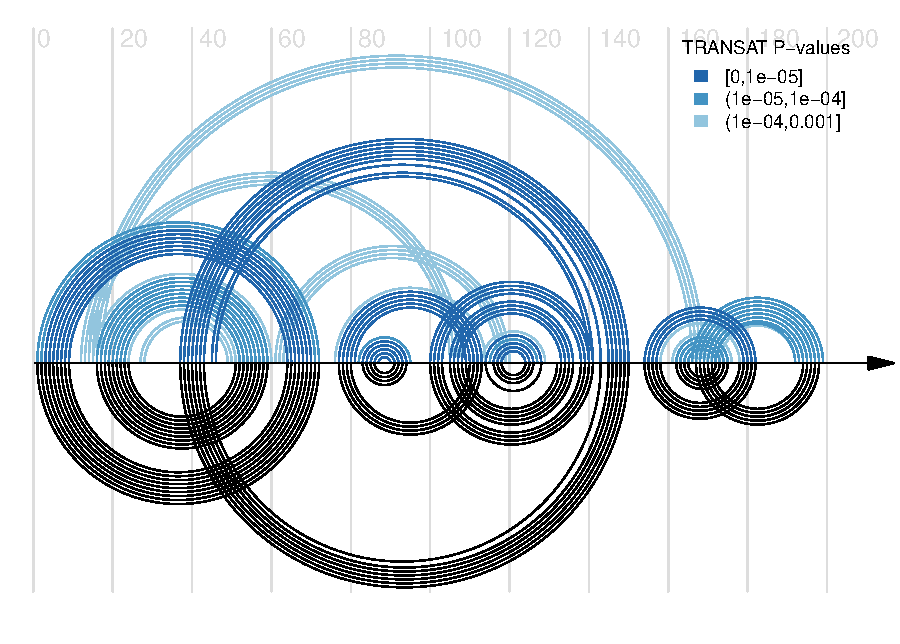
\includegraphics{R4RNA-010}

Same can be done to multiple entitites.

\begin{Schunk}
\begin{Sinput}
> helix.transat.exp <- helix.transat.exp[,1:6]
> helix.transat.exp$col <- col <- colourByValueMltp(helix.transat.exp, log = TRUE)
> message("Coloured encoded in 'col' column of transat structure")
> plotDoubleHelixMltpSingleLine(helix.known.exp,helix.transat.exp,scale = FALSE)
> legend("topright", legend = attr(col, "legend"), fill = attr(col, "fill"),
+ 	inset = 0.05, bty = "n", border = NA, cex = 0.75, title = "TRANSAT P-values")
\end{Sinput}
\end{Schunk}
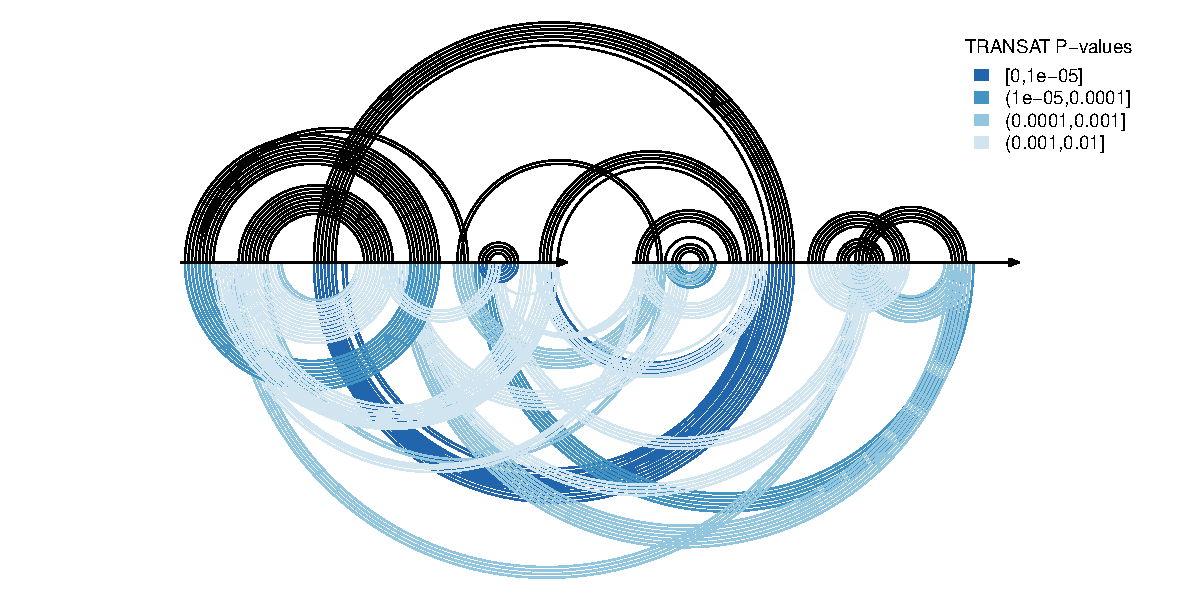
\includegraphics{R4RNA-011}

\begin{Schunk}
\begin{Sinput}
> helix.transat.exp <- helix.transat.exp[,1:6]
> helix.transat.exp$col <- col <- colourByValueMltp(helix.transat.exp, log = TRUE)
> message("Coloured encoded in 'col' column of transat structure")
> plotDoubleHelixMltpDoubleLine(helix.known.exp,helix.transat.exp,scale = FALSE,stable = TRUE)
> legend("topright", legend = attr(col, "legend"), fill = attr(col, "fill"),
+ 	inset = 0.05, bty = "n", border = NA, cex = 0.75, title = "TRANSAT P-values")
\end{Sinput}
\end{Schunk}
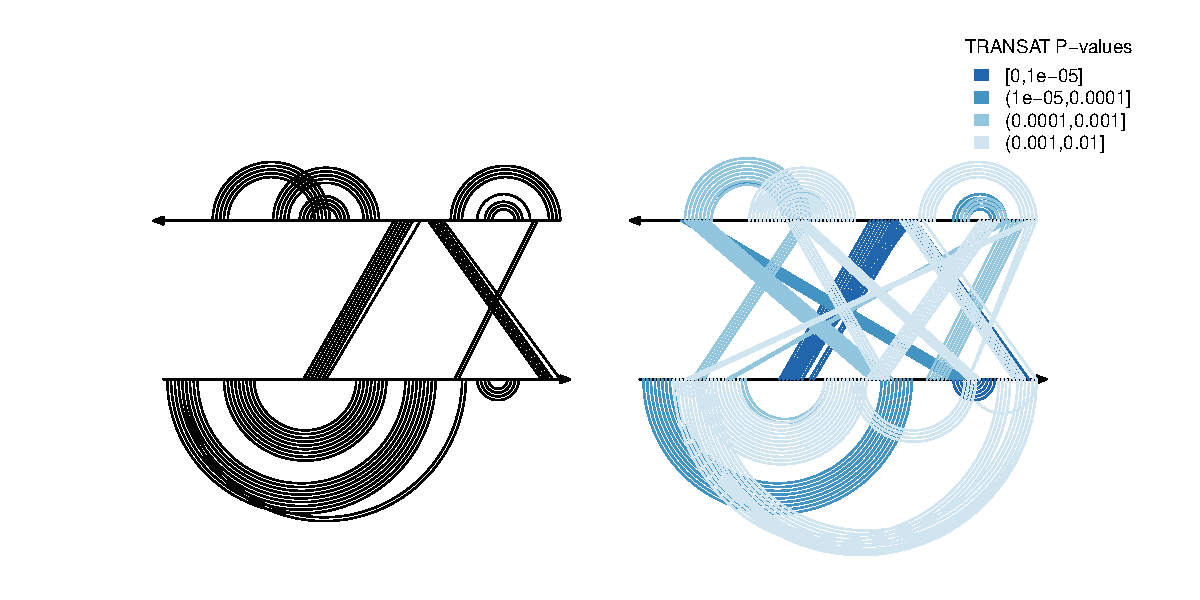
\includegraphics{R4RNA-012}


\subsection{Overlapping Multiple Structures}

A neat way of visualizing the concordance between two structure is an
overlapping structure diagram, which we can use to overlap the predicted TRANSAT
structure and the known RFAM structure.  Predicted basepairs that exist in the
known structure are drawn above the line, and those predicted that are not known
to exist are drawn below.  Those known but unpredicted are shown in black above
the line.

\begin{Schunk}
\begin{Sinput}
> plotOverlapHelix(transat, known, line = TRUE, arrow = TRUE, scale = FALSE)
\end{Sinput}
\end{Schunk}
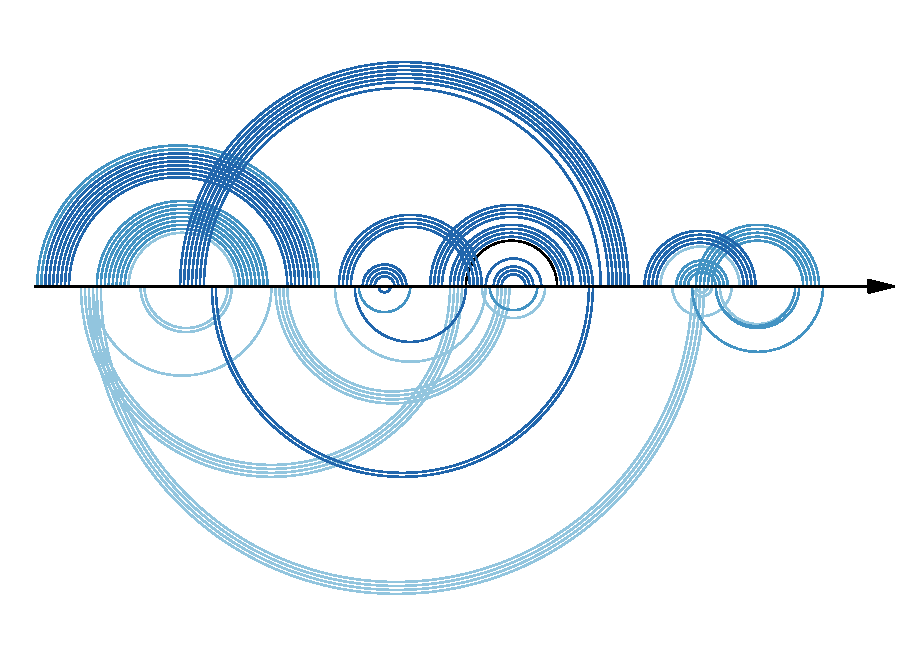
\includegraphics{R4RNA-013}

Same can be done to multiple entitites.

\begin{Schunk}
\begin{Sinput}
> plotComparisonHelixMltpSingleLine(helix1 = helix.known.exp[,1:6],
+                                   helix2 = helix.transat.exp[,1:6],
+                                   scale = FALSE)
> mtext("Known Structure", side = 3, line = -5, adj = 0)
> mtext("Predicted\nStructure", side = 1, line = -2, adj = 0)
\end{Sinput}
\end{Schunk}
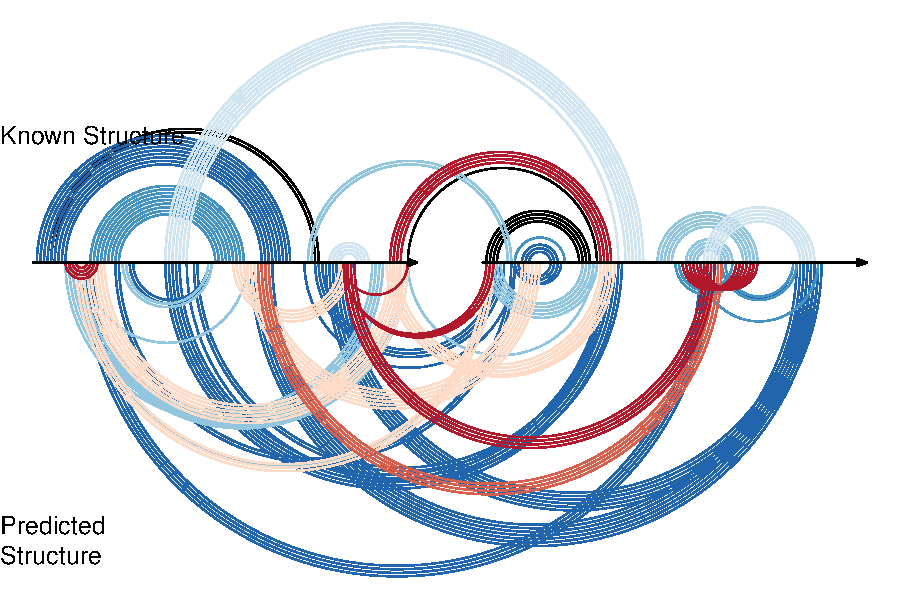
\includegraphics{R4RNA-014}

\begin{Schunk}
\begin{Sinput}
> plotComparisonHelixMltpDoubleLine(helix1 = helix.known.exp[,1:6],
+                                   helix2 = helix.transat.exp[,1:6],
+                                   scale = FALSE)
> mtext("Known Structure", side = 3, line = -5, adj = 0)
> mtext("Predicted\nStructure", side = 1, line = -2, adj = 0)
\end{Sinput}
\end{Schunk}
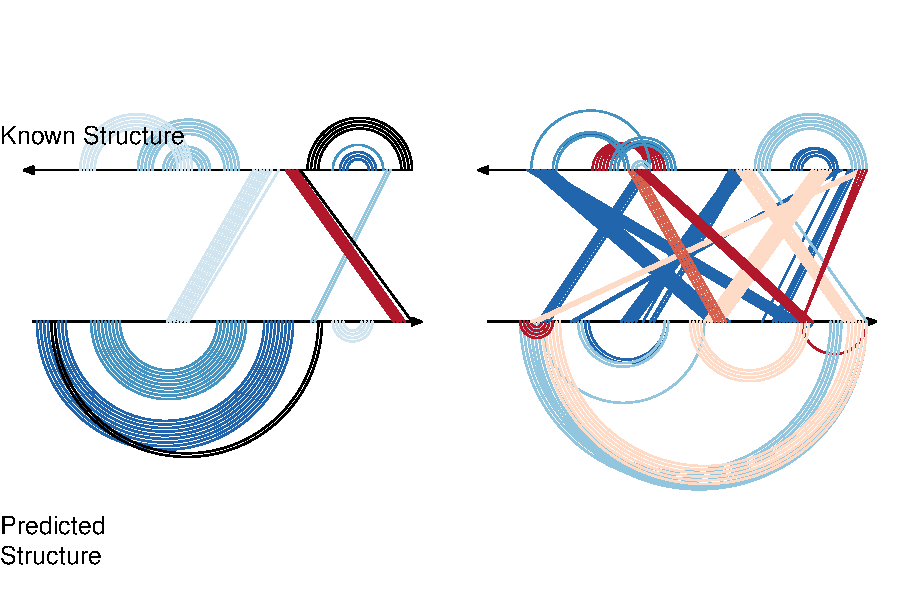
\includegraphics{R4RNA-015}

\subsection{Visualizing Multiple Sequence Alignments}

In addition to visualizing the structure alone, we can also visualize a
secondary structure along with aligned nucleotide sequences.  In the following,
we will read in a multiple sequence alignment obtained from RFAM, and visualize
the known structure on top of it.

We can also annotate the alignment colours according to their agreement with the
known structure.  If a sequence can form as basepair as dictated by the structure,
the basepair is coloured green, else red.  For green basepairs, if a mutation
has occured, but basepairing potential is retained, it is coloured in blue
(dark for mutations in both bases, light for single-sided mutation).  Unpaired
bases are in black and gaps are in grey.

\begin{Schunk}
\begin{Sinput}
> message("Multiple sequence alignment of interest")
> library(Biostrings)
> fasta_file <- system.file("extdata", "fasta.txt", package = "R4RNA")
> fasta <- as.character(readBStringSet(fasta_file))
> message("Plot covariance in alignment")
> plotCovariance(fasta, known, cex = 0.5)
\end{Sinput}
\end{Schunk}
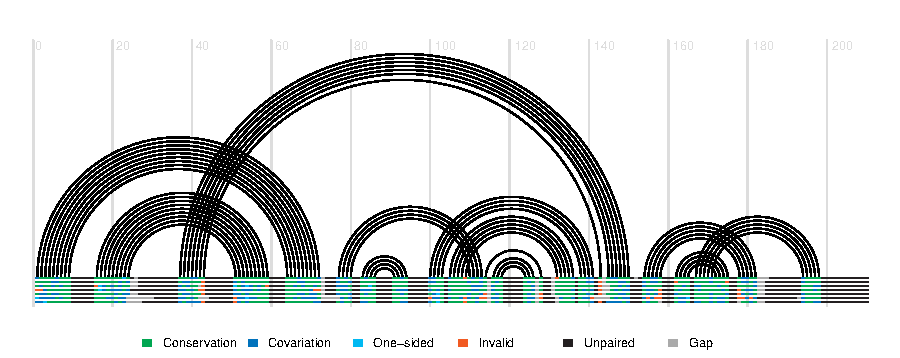
\includegraphics{R4RNA-016}

Same can be done to multiple entitites.

\begin{Schunk}
\begin{Sinput}
> message("Multiple sequence alignment of interest")
> fasta_file.mltp <- system.file("extdata", "fasta.mltp.txt", package = "R4RNA")
> fasta.mltp <- readBStringSet(fasta_file.mltp)
> message("Plot covariance in alignment")
> plotCovarianceMltpSingleLine(helix = helix.transat.exp[,1:7],
+                              msa = fasta.mltp,grid = FALSE,
+                              scale = FALSE)
\end{Sinput}
\end{Schunk}
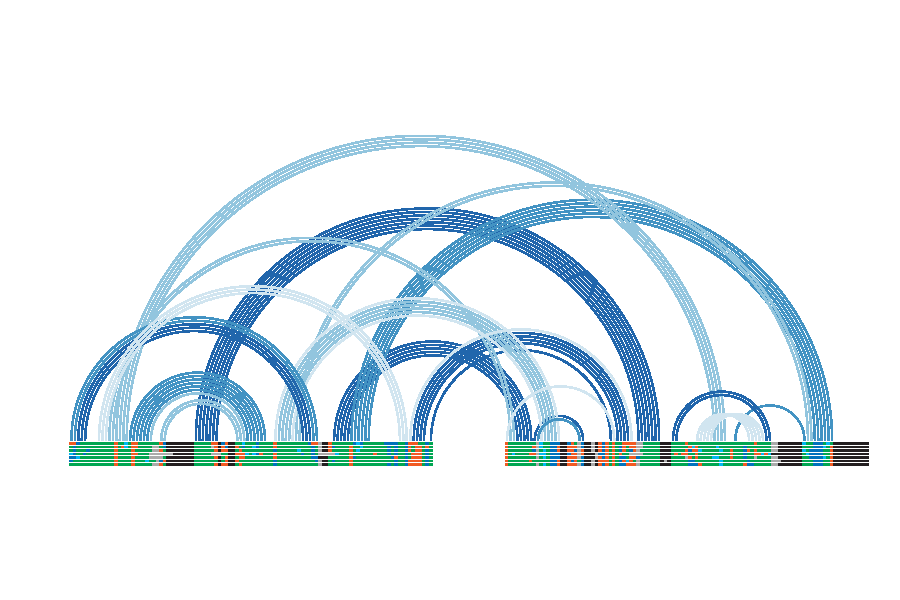
\includegraphics{R4RNA-017}


\begin{Schunk}
\begin{Sinput}
> message("Multiple sequence alignment of interest")
> fasta_file.mltp <- system.file("extdata", "fasta.mltp.txt", package = "R4RNA")
> fasta.mltp <- readBStringSet(fasta_file.mltp)
> message("Plot covariance in alignment")
> plotCovarianceMltpDoubleLine(helix = helix.transat.exp[,1:7],
+                              msa = fasta.mltp,grid = FALSE,
+                              legend = FALSE,scale = FALSE)
\end{Sinput}
\end{Schunk}

\includegraphics{R4RNA-018}

\subsection{Overlapping Multiple Structures with Multiple Sequence Alignments}

Overlapping Multiple Structures can be presented with msa and have msa
annotation. There is 3 functions for it. They follow same rules as usual
comparison does. Predicted basepairs that exist in the known structure are drawn
above the line, and those predicted that are not known to exist are drawn below.
Those known but unpredicted are shown in black above the line.

Single Line mode where upper and bottom part shares same msa visualization.

\begin{Schunk}
\begin{Sinput}
> plotCovarianceComparisonMltpSingleLine(msa = fasta.mltp,
+                                        helix1 = helix.known.exp[,1:6],
+                                        helix2 = helix.transat.exp[,1:6],
+                                        scale = FALSE,legend = FALSE,
+                                        species = 0)
> 
\end{Sinput}
\end{Schunk}
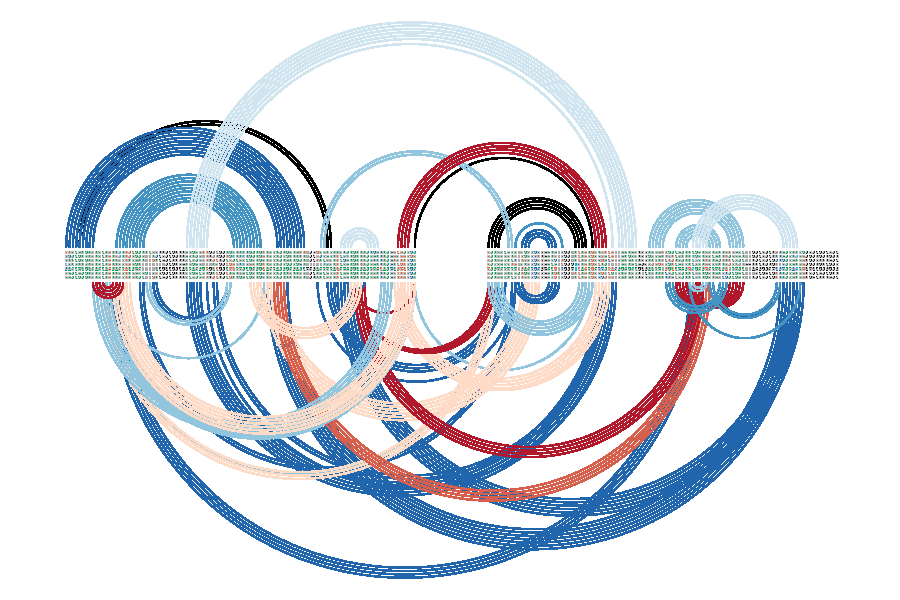
\includegraphics{R4RNA-019}

Single Line mode where upper and bottom part have their own msa visualization.

\begin{Schunk}
\begin{Sinput}
> plotDoubleCovarianceComparisonMltpSingleLine(msa = fasta.mltp,
+                                              helix1 = helix.known.exp[,1:6],
+                                              helix2 = helix.transat.exp[,1:6],
+                                              scale = FALSE,legend = FALSE,
+                                              species = 0,dist.y.between = 5 )
\end{Sinput}
\end{Schunk}
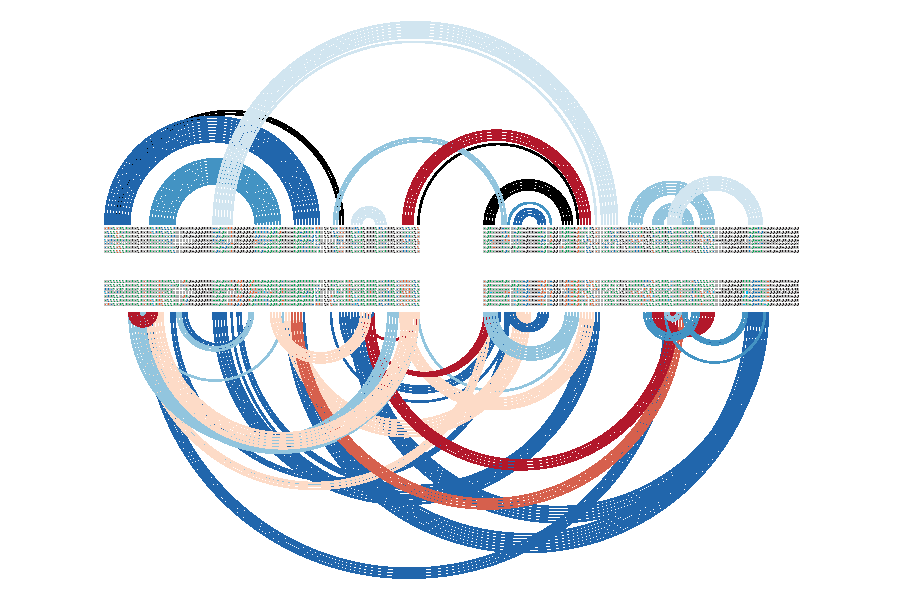
\includegraphics{R4RNA-020}

Double Line mode where predicted basepairs that exist in the known structure are drawn
on left side, and those predicted that are not known to exist are drawn on right side.
Those known but unpredicted are shown in black on left side.
\begin{Schunk}
\begin{Sinput}
> plotCovarianceComparisonMltpDoubleLine(msa = fasta.mltp,
+                                        helix1 = helix.known.exp[,1:6],
+                                        helix2 = helix.transat.exp[,1:6],
+                                        scale = FALSE,legend = FALSE,
+                                        species = 0)
\end{Sinput}
\end{Schunk}
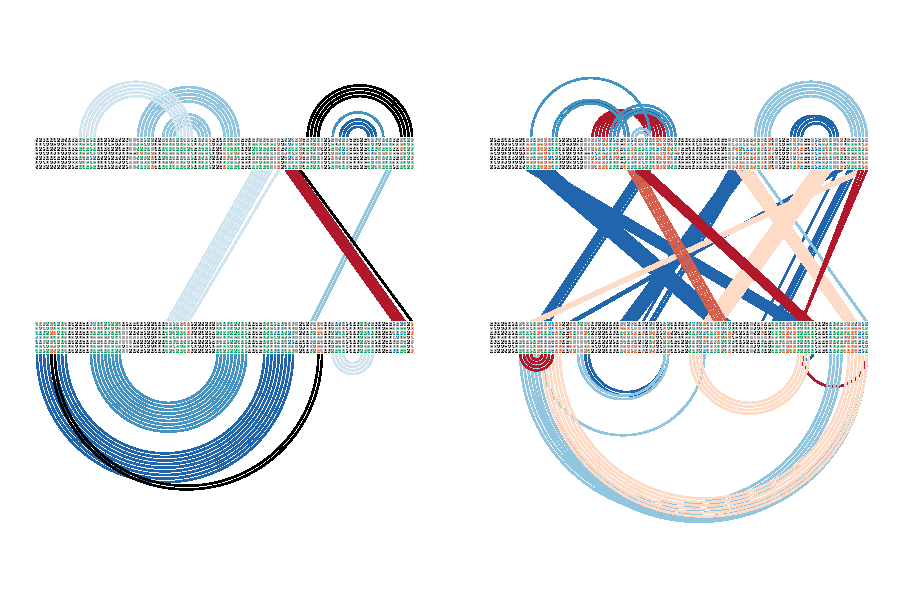
\includegraphics{R4RNA-021}


\subsection{Multiple Sequence Alignements with Annotated Arcs}

Arcs can be coloured as usual.  It should be noted that structures with
conflicting basepairs (arcs sharing a base) cannot be visualized properly
on a multiple sequence alignment, and are typically filtered out (\textit{e.g.}
drawn in grey here).

\begin{Schunk}
\begin{Sinput}
> plotCovariance(fasta, transat, cex = 0.5, conflict.col = "grey")
\end{Sinput}
\end{Schunk}
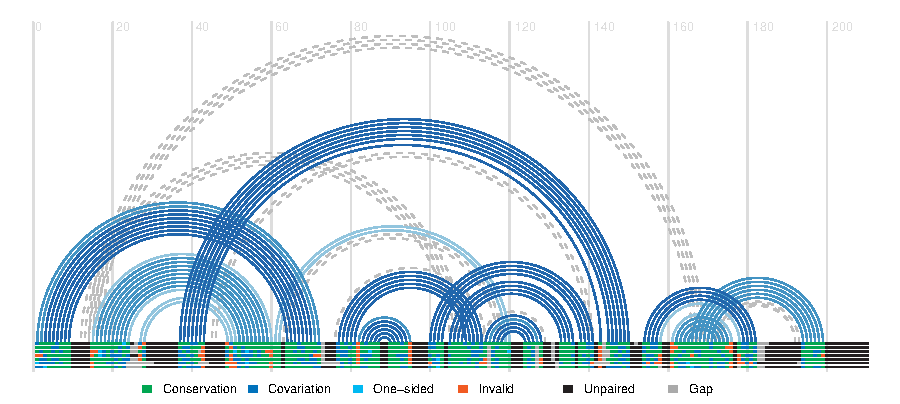
\includegraphics{R4RNA-022}

Same can be done to multiple entitites.

\begin{Schunk}
\begin{Sinput}
> message("Multiple sequence alignment of interest")
> fasta_file.mltp <- system.file("extdata", "fasta.mltp.txt", package = "R4RNA")
> fasta.mltp <- readBStringSet(fasta_file.mltp)
> message("Plot covariance in alignment")
> plotCovarianceMltpSingleLine(helix = helix.transat.exp[,1:7],msa = fasta.mltp,
+                              conflict.col = "grey",legend = TRUE,grid = FALSE,scale = FALSE)
\end{Sinput}
\end{Schunk}
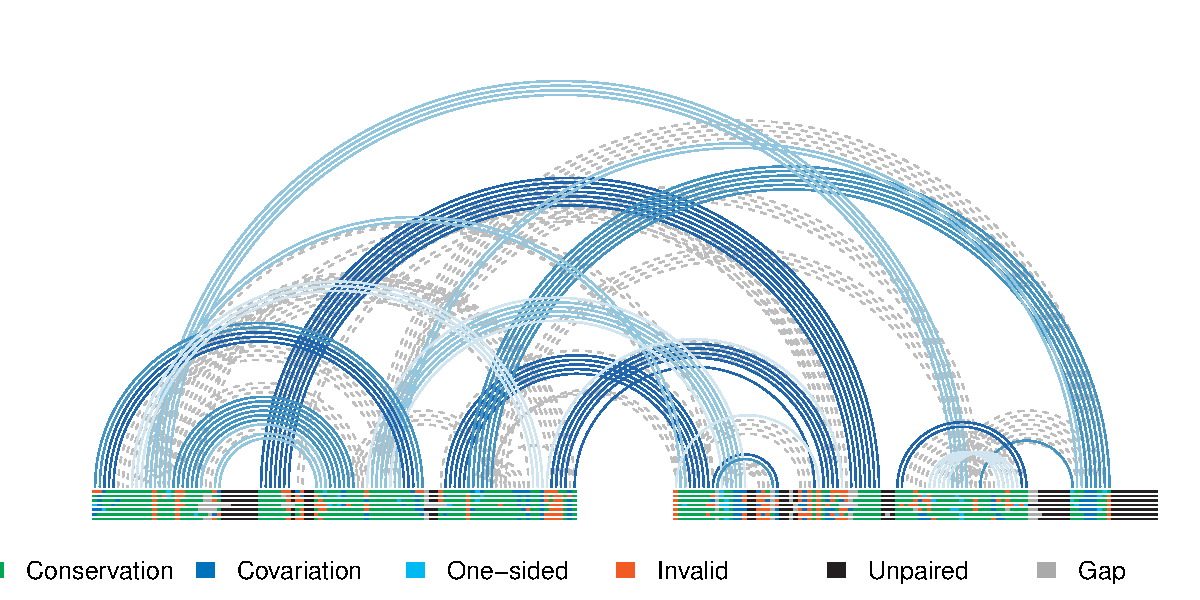
\includegraphics{R4RNA-023}

\begin{Schunk}
\begin{Sinput}
> message("Multiple sequence alignment of interest")
> fasta_file.mltp <- system.file("extdata", "fasta.mltp.txt", package = "R4RNA")
> fasta.mltp <- readBStringSet(fasta_file.mltp)
> message("Plot covariance in alignment")
> plotCovarianceMltpDoubleLine(helix = helix.transat.exp[,1:7],msa = fasta.mltp,
+                              conflict.col = "grey",grid = FALSE,scale = FALSE)
\end{Sinput}
\end{Schunk}
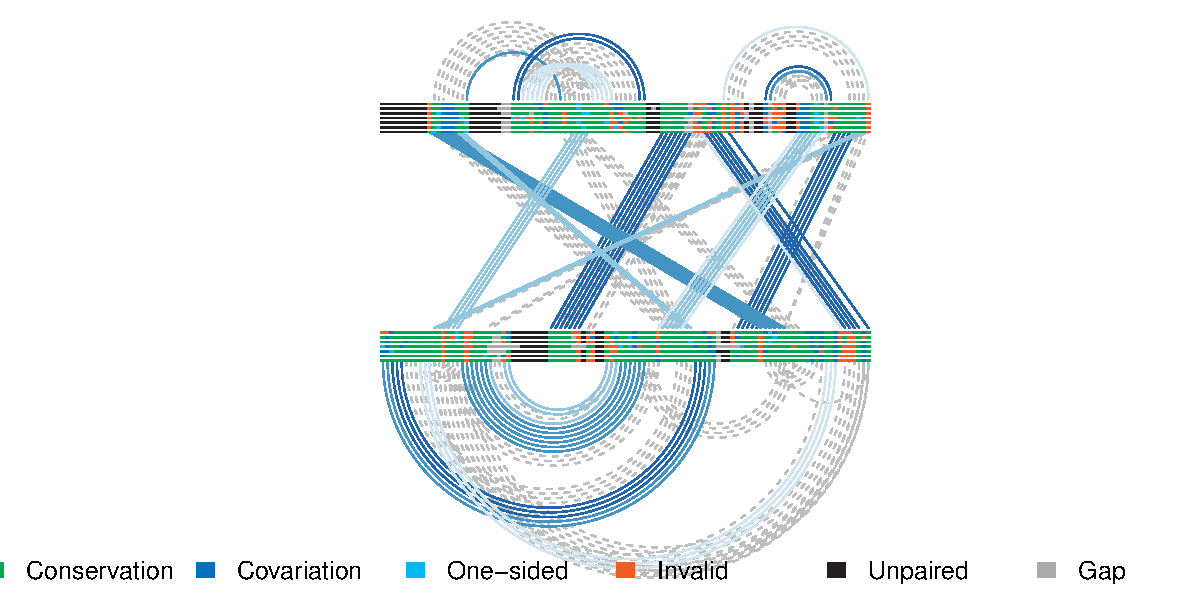
\includegraphics{R4RNA-024}


\subsection{Additional Colouring Methods}

Various other methods of colour arcs exist, along with many options to control
appearances:

\subsubsection{Colour By Covariation (with alignment as blocks)}

\begin{Schunk}
\begin{Sinput}
> col <- colourByCovariation(known, fasta, get = TRUE)
> plotCovariance(fasta, col, grid = TRUE, legend = FALSE)
> legend("topright", legend = attr(col, "legend"), fill = attr(col, "fill"),
+     inset = 0.1, bty = "n", border = NA, cex = 0.37, title = "Covariation")
\end{Sinput}
\end{Schunk}
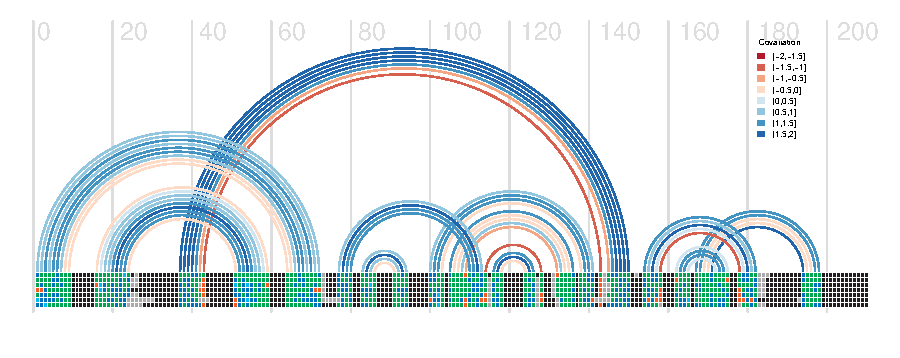
\includegraphics{R4RNA-025}

\begin{Schunk}
\begin{Sinput}
> col <- colourByCovariationMltp(helix = helix.transat.exp,msa = fasta.mltp,get = TRUE)
> plotCovarianceMltpSingleLine(helix = col,msa = fasta.mltp,grid = TRUE,scale = FALSE)
> legend("topright", legend = attr(col, "legend"), fill = attr(col, "fill"),
+        inset = 0.1, bty = "n", border = NA, cex = 0.5, title = "Covariation")
\end{Sinput}
\end{Schunk}
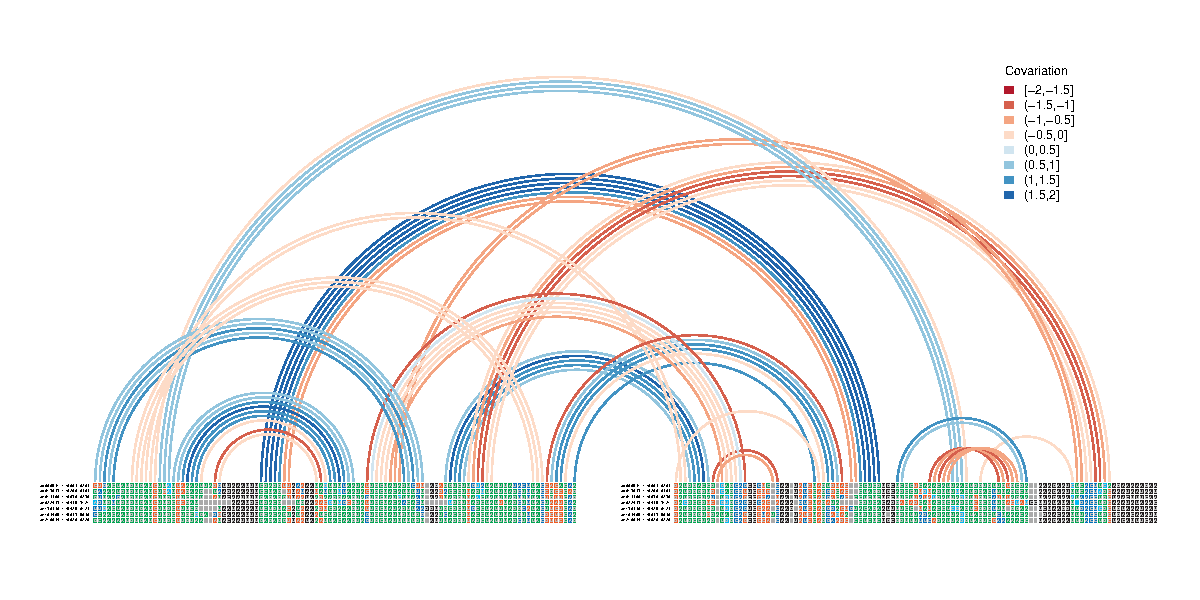
\includegraphics{R4RNA-026}


\subsubsection{Colour By Conservation (with custom alignment colours)}

\begin{Schunk}
\begin{Sinput}
> custom_colours <- c("green", "blue", "cyan", "red", "black", "grey")
> plotCovariance(fasta, col <- colourByConservation(known, fasta, get = TRUE),
+     palette = custom_colours, cex = 0.5)
> legend("topright", legend = attr(col, "legend"), fill = attr(col, "fill"),
+     inset = 0.15, bty = "n", border = NA, cex = 0.75, title = "Conservation")
\end{Sinput}
\end{Schunk}
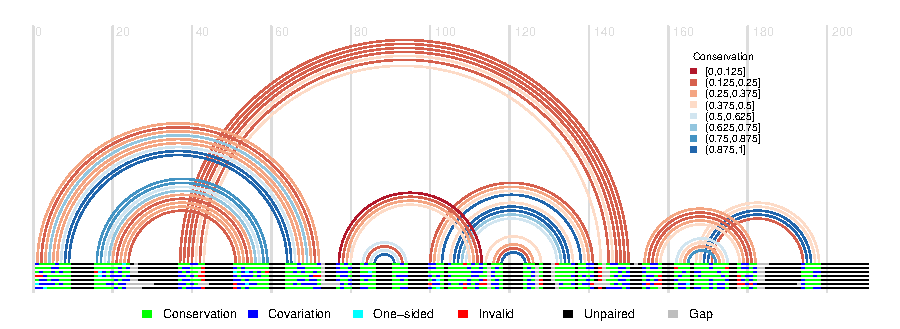
\includegraphics{R4RNA-027}

\begin{Schunk}
\begin{Sinput}
> custom_colours <- c("green", "blue", "cyan", "red", "black", "grey")
> plotCovarianceMltpSingleLine(msa = fasta.mltp,
+                              helix = col <- colourByConservationMltp(helix = helix.transat.exp,
+                                                                      msa = fasta.mltp,get = TRUE,
+                                                                      cols = custom_colours),
+                              palette = custom_colours,scale = FALSE)
> legend("topright", legend = attr(col, "legend"), fill = attr(col, "fill"),
+ 	inset = 0.15, bty = "n", border = NA, cex = 0.75, title = "Conservation")
\end{Sinput}
\end{Schunk}
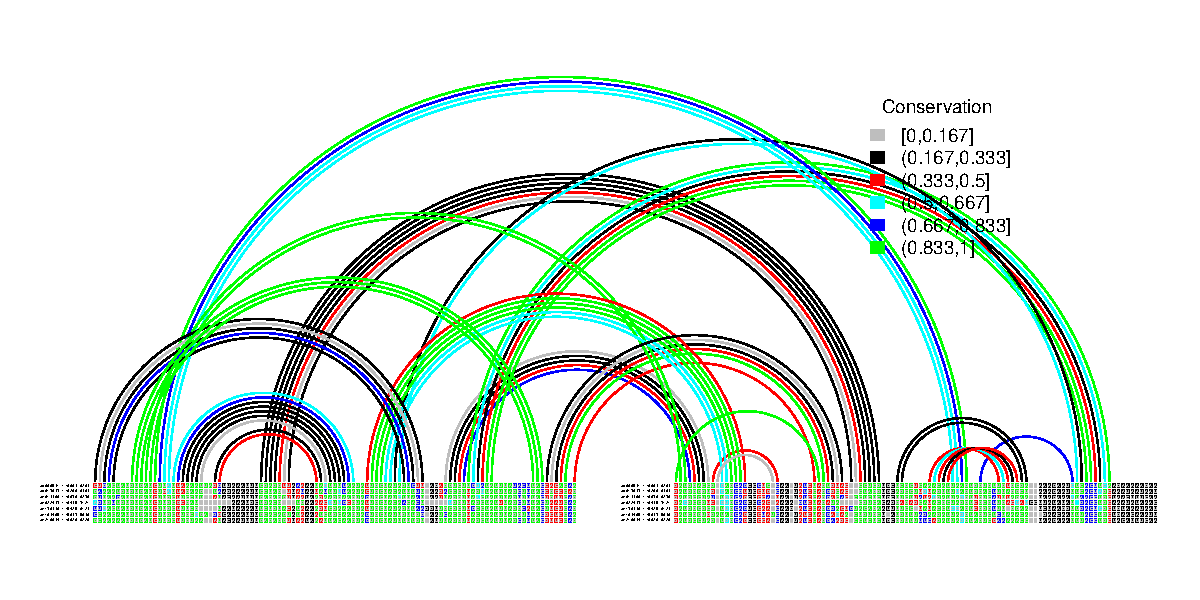
\includegraphics{R4RNA-028}


\subsubsection{Colour By Percentage Canonical Basepairs (with custom arc colours)}

\begin{Schunk}
\begin{Sinput}
> col <- colourByCanonical(known, fasta, custom_colours, get = TRUE)
> plotCovariance(fasta, col, base.colour = TRUE, cex = 0.5)
> legend("topright", legend = attr(col, "legend"), fill = attr(col, "fill"),
+     inset = 0.15, bty = "n", border = NA, cex = 0.75, title = "% Canonical")
\end{Sinput}
\end{Schunk}
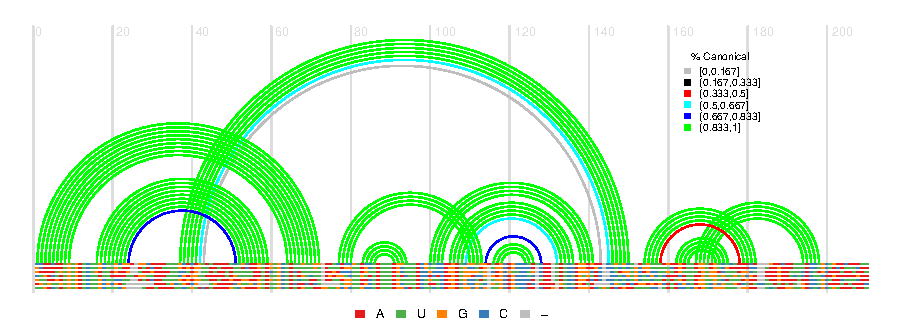
\includegraphics{R4RNA-029}

\begin{Schunk}
\begin{Sinput}
> col <- colourByCanonicalMltp(helix = helix.transat.exp,msa = fasta.mltp,get = TRUE)
> plotCovarianceMltpSingleLine(helix = col,msa = fasta.mltp,scale = FALSE)
> legend("topright", legend = attr(col, "legend"), fill = attr(col, "fill"),
+ 	inset = 0.15, bty = "n", border = NA, cex = 0.75, title = "% Canonical")
\end{Sinput}
\end{Schunk}
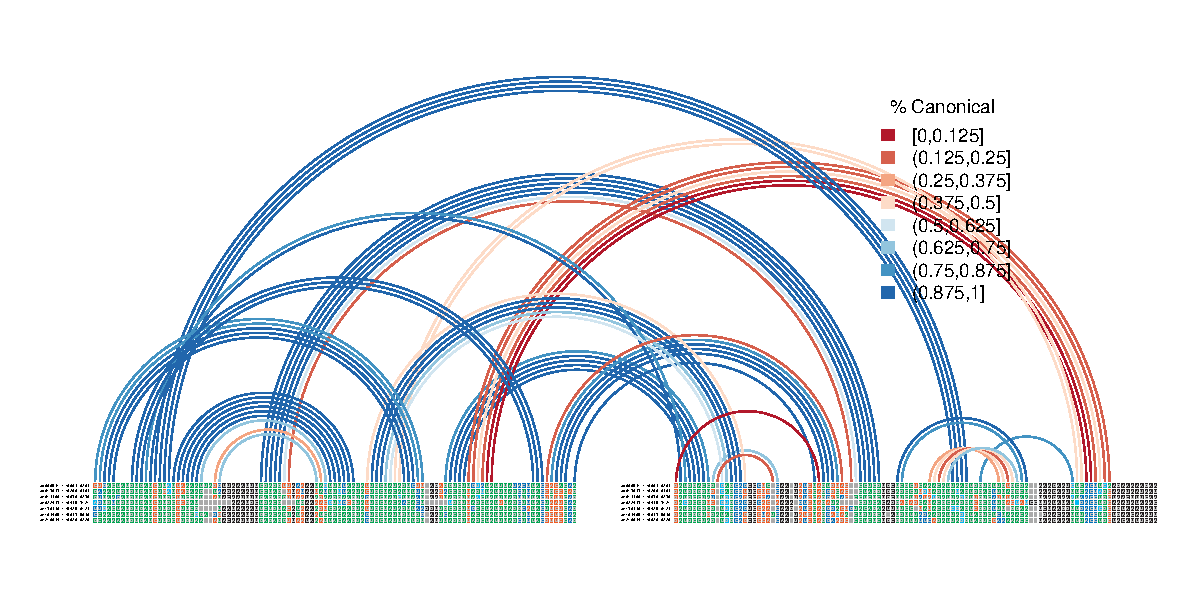
\includegraphics{R4RNA-030}


\subsubsection{Colour Pseudoknots (with CLUSTALX-style alignment)}

\begin{Schunk}
\begin{Sinput}
> col <- colourByUnknottedGroups(known, c("red", "blue"), get = TRUE)
> plotCovariance(fasta, col, base.colour = TRUE, legend = FALSE,
+                species = 23, grid = TRUE, text = TRUE,
+                text.cex = 0.2, cex = 0.5)
\end{Sinput}
\end{Schunk}
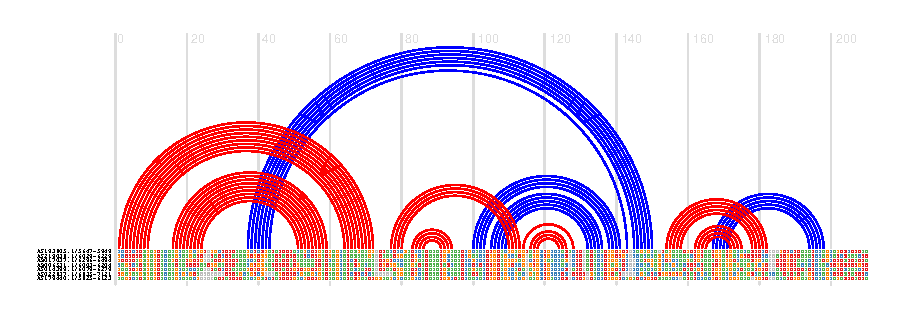
\includegraphics{R4RNA-031}

\begin{Schunk}
\begin{Sinput}
> col <- colourByUnknottedGroupsMltp(helix = helix.transat.exp,cols = c("red","blue"),get = TRUE)
> plotCovarianceMltpSingleLine(helix = col,msa = fasta.mltp,base.colour = TRUE,scale = FALSE)
\end{Sinput}
\end{Schunk}
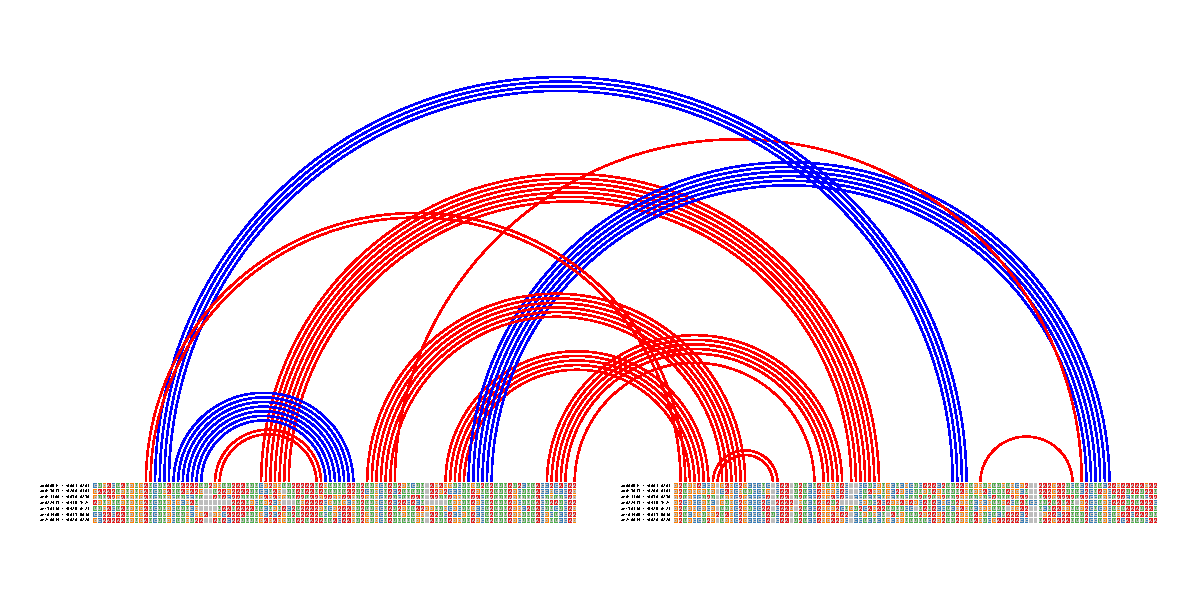
\includegraphics{R4RNA-032}

\subsection{Working with HiC data}

HiC triangular format file obtained with straw

\begin{Schunk}
\begin{Sinput}
> hic_file <- system.file("extdata", "GSE63525.chr10.chr11.500kb.txt", package = "R4RNA")
> helix_hic <- StrawToHelix(file = hic_file, chr1 = "chr10",chr2 = "chr11",scale = 500000)
\end{Sinput}
\end{Schunk}


Trimm low values of strength interactions. After update attribute for new generated helix file. And colour by value (interaction strength).

\begin{Schunk}
\begin{Sinput}
> helix_hic.trimmed <- helix_hic[value > 40]
> attr(helix_hic.trimmed,"length") <- attr(helix_hic,"length")
> helix_hic.trimmed <- colourByValueMltp(helix_hic.trimmed,get = TRUE)
\end{Sinput}
\end{Schunk}

Plot figure from filtered data

\begin{Schunk}
\begin{Sinput}
> plotHelixMltpSingleLine(helix = helix_hic.trimmed,shape = "triangle",scale = FALSE)
\end{Sinput}
\end{Schunk}
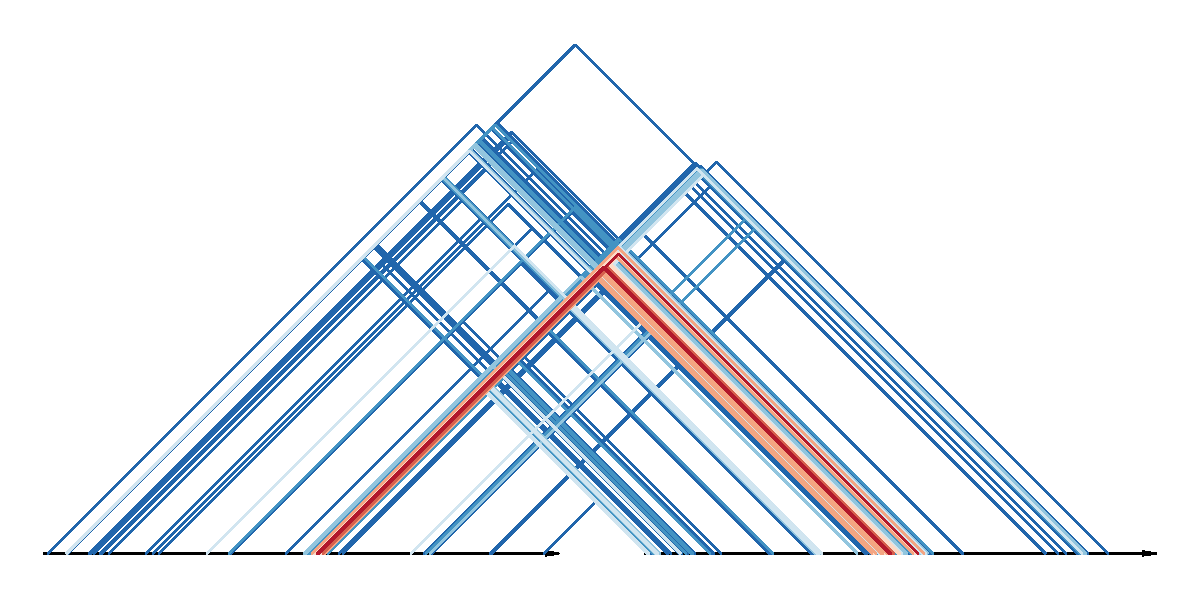
\includegraphics{R4RNA-035}

Plot figure from filtered data in heatmap way

\begin{Schunk}
\begin{Sinput}
> plotHelixMltpSingleLine(helix = helix_hic.trimmed,shape = "heatmap",scale = FALSE)
\end{Sinput}
\end{Schunk}
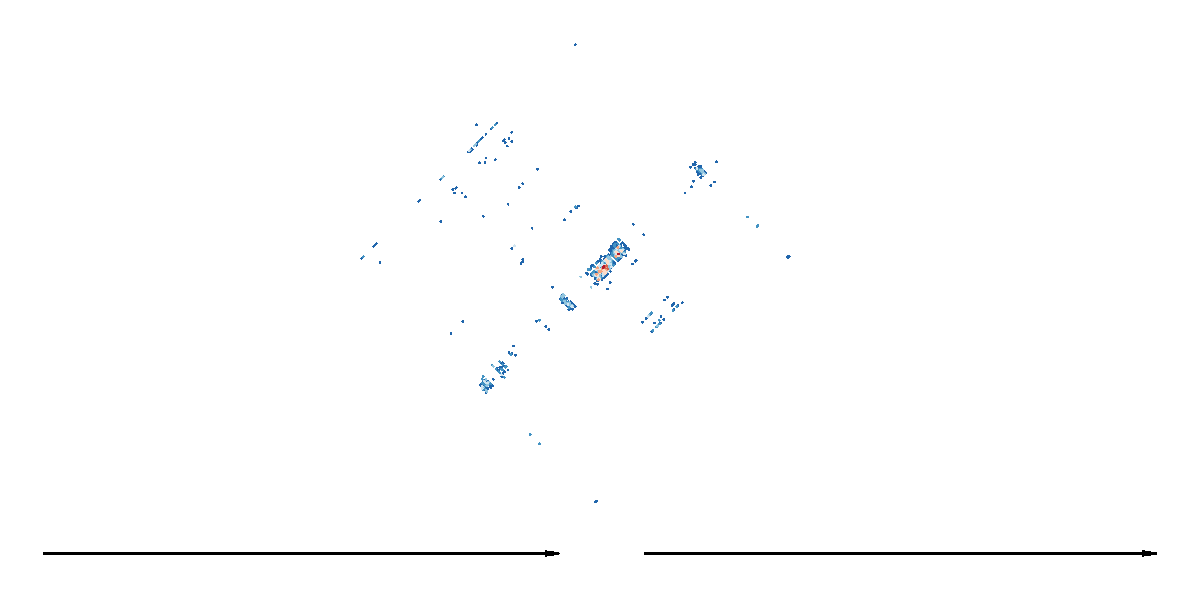
\includegraphics{R4RNA-036}

\section{Session Information}

The version number of R and packages loaded for generating the vignette were:

\begin{itemize}\raggedright
  \item R version 3.6.3 (2020-02-29), \verb|x86_64-w64-mingw32|
  \item Locale: \verb|LC_COLLATE=Russian_Russia.1251|, \verb|LC_CTYPE=Russian_Russia.1251|, \verb|LC_MONETARY=Russian_Russia.1251|, \verb|LC_NUMERIC=C|, \verb|LC_TIME=Russian_Russia.1251|
  \item Running under: \verb|Windows 10 x64 (build 18363)|
  \item Matrix products: default
  \item Base packages: base, datasets, graphics, grDevices, methods,
    parallel, stats, stats4, utils
  \item Other packages: BiocGenerics~0.32.0, Biostrings~2.54.0,
    data.table~1.12.8, IRanges~2.20.2, R4RNA~2.0.8, S4Vectors~0.24.3,
    XVector~0.26.0
  \item Loaded via a namespace (and not attached): compiler~3.6.3,
    tools~3.6.3, zlibbioc~1.32.0
\end{itemize}
\end{document}
